\chapter{Design} \label{chap:design}
This chapter covers the design of the blockchain explorer and the additional components necessary to run the application.

\section{Structure of the Service}
The program that users and admins use to view blockchain data is a website, which is made up of a front- and a backend. However, to run the blockchain explorer on its own, additional components beside the front- and backend programs are required. The website fetches blockchain data from an SQL database that runs independently from the blockchain. A separate database was chosen, because additional data like statistical information needs to be calculated and stored as well, which would bloat all miner?s built-in databases with information, if implemented in the miner. The fact that there are unified data structures and the possibility of having stored procedures in the database makes SQL a preferable database model, since the website always queries predefined statements. This also makes running the website possible without having a miner running in the backend. However this requires a program that copies data from a running Bazo mining node's database and stores it in the new  SQL database. As mentioned above, the backend accesses this database by making queries for relevant data and sending the results to the frontend to be displayed to the user.
GRAPHIC OF SYSTEM
\section{Structure of the Website}
\section{idk}
\begin{figure}
  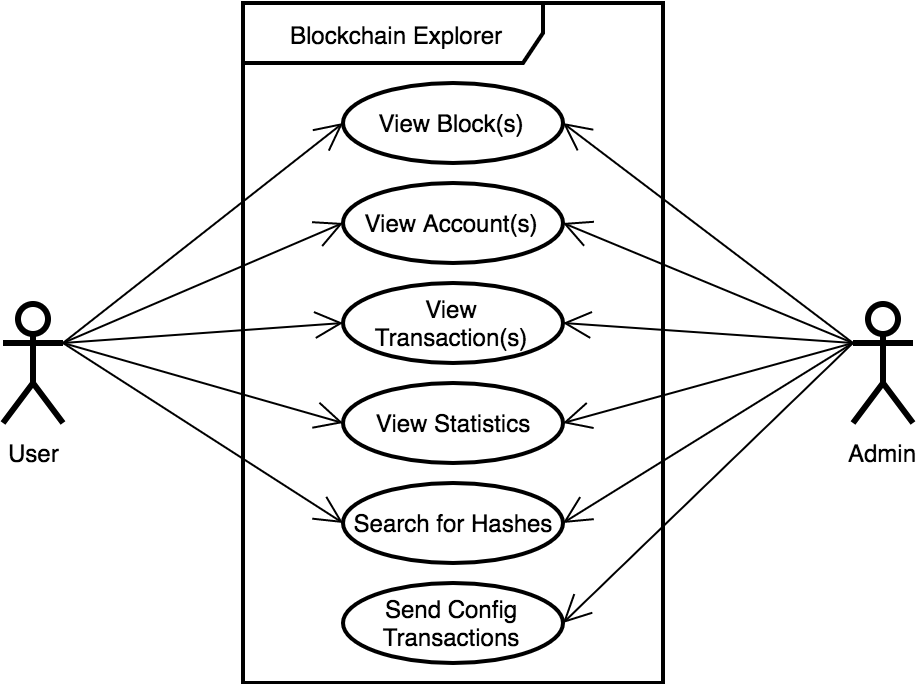
\includegraphics[width=\linewidth]{usecase1.png}
  \caption{Use Cases of the Block Explorer}
  \label{fig:usecase1}
\end{figure}

\chapter{Implementation}
This chapter documents the implementation of the components listed in chapter \ref{chap:design}; Frontend, Backend and the SQL database. An additional section concerning hosting of the application on the internet is also included.
\section{Frontend}
XXX
\subsection{HTML-Templates}
To interact with the Golang-Backend of the application, Gohtml templates have been used to define the markup of the application. One one hand, this makes way for a modular view component by letting programmers define reusable HTML modules such as headers, footers or table-templates. Using templates can minimize code duplication, which in turn makes maintenance on the code an overall less risky task. On the other hand, Golang templates allow for some limited logic in the Gohtml files, which is needed for handling variables that get passed from the backend component. For example, if the passed variable is an array of integers and the goal is to display all variables in a list, golang can create a new <li> tag for every value in the array. The HTML code that gets passed to the end user after making a request contains no Golang code, since the backend renders the Gohtml template files and passed variables to a useable HTML file that can be displayed by a web browser. Except for some Bootstrap functionality mentioned in \ref{sec:uiframeworks} and one case discussed in section \ref{sec:clientside}, all rendered pages of the application are static HTML files, because for every action a user may make on the website, a request has to be made to the backend. The website aims to always display the most recent data, so storing information that may not be up to date on the client's machine in order to save bandwidth, is outweighed by the possibility of having more recent data. 

\subsection{UI Frameworks} \label{sec:uiframeworks}
\subsection{Client-Side Logic} \label{sec:clientside}